\documentclass[11pt,a4paper]{article}

% ---------------------------------------------------------------- packages
\usepackage[T1]{fontenc}
\usepackage[utf8]{inputenc}
\usepackage{lmodern}
\usepackage[margin=2.6cm]{geometry}
\usepackage{microtype}
\usepackage{amsmath,amssymb,amsthm}
\usepackage{graphicx}
\usepackage{booktabs}
\usepackage{xcolor}
\usepackage{enumitem}
\usepackage{caption}
\usepackage{algorithm}
\usepackage{algpseudocode}
\usepackage{listings}
\usepackage{url}
\usepackage[colorlinks=true,linkcolor=linkblue,citecolor=linkblue,urlcolor=linkblue]{hyperref}
\usepackage[capitalise,noabbrev]{cleveref}

\definecolor{linkblue}{HTML}{1C5CAB}
\hypersetup{pdftitle={The Potapov-Grishin Principal Hyperface Method, Completed and Machine-Checked},pdfauthor={O. Bodnar}}
\definecolor{codebg}{HTML}{F5F7FA}
\captionsetup{font=small,labelfont=bf,margin=1em}
\setlist{itemsep=2pt,topsep=4pt}
\linespread{1.05}

\lstset{basicstyle=\ttfamily\small,backgroundcolor=\color{codebg},frame=single,
  rulecolor=\color{codebg},xleftmargin=1em,xrightmargin=1em,columns=fullflexible,
  keepspaces=true,showstringspaces=false}

\theoremstyle{plain}
\newtheorem{theorem}{Theorem}
\newtheorem{lemma}[theorem]{Lemma}
\newtheorem{corollary}[theorem]{Corollary}
\newtheorem{proposition}[theorem]{Proposition}
\theoremstyle{definition}
\newtheorem{definition}[theorem]{Definition}
\theoremstyle{remark}
\newtheorem*{remark}{Remark}

\newcommand{\R}{\mathbb{R}}
\newcommand{\K}{\mathbb{K}}
\newcommand{\lean}[1]{\texttt{\small #1}}
\newcommand{\repourl}{\url{https://github.com/albond/principal-hyperfaces}}

\title{\textbf{The Potapov--Grishin Principal Hyperface Method,\\Completed and Machine-Checked}\\[6pt]
\large Correctness, existence of principal hyperfaces, an exact selection rule in the plane,\\
and a certified algorithm for linear programming verified in Lean~4}
\author{O.~Bodnar\\[2pt]\small Independent Researcher\\
\small ORCID: \href{https://orcid.org/0009-0007-9716-1853}{0009-0007-9716-1853}}
\date{2026}

\begin{document}
\maketitle

\begin{abstract}
\noindent
The principal hyperface method of G.\,G.~Potapov and I.\,Yu.~Grishin (2007) solves a linear
program by a sequence of geometric decisions. It picks the constraint hyperplane whose normal
is closest in direction to the objective vector, turns that inequality into an equality,
eliminates one variable, and repeats, so that the dimension drops by one at each step. The
method is short and easy to picture, but it was published as a heuristic, without a proof of
when it is correct.

This paper completes the method and verifies every result in the Lean~4 proof assistant. We
prove that a run of the method returns an optimal point \emph{if and only if} every hyperface
it selects is \emph{principal}, that is, active at some optimum. We prove that a principal
hyperface always exists when the objective is non-zero. We prove that in two dimensions the
projection rule of the method never errs on systems without redundant constraints, and we give
a machine-checked counterexample in three dimensions. Finally, we turn the method into a
\emph{certified} algorithm: it follows the projection rule, checks a dual certificate after
each step, and backtracks when the check fails. We prove that it always returns an optimal point
when one exists, and every certified answer can be checked independently. Along the way we
formalise Farkas' lemma over an arbitrary ordered field by Fourier--Motzkin elimination. The
worked example of the 2008 paper is confirmed exactly. A Python implementation of the same
algorithm in exact rational arithmetic accompanies the paper.
\end{abstract}

\medskip
\noindent\textbf{Keywords:} linear programming; principal hyperfaces; Farkas' lemma;
Fourier--Motzkin elimination; certified algorithms; formal verification; Lean~4.

% =====================================================================
\section{Introduction}\label{sec:intro}

A linear program asks for the largest value of a linear function $c\cdot x$ over a convex
polyhedron $P=\{x : a_i\cdot x\le b_i\}$. The optimum, when it exists, sits on the boundary of
$P$, where some of the inequalities hold with equality. The simplex method of
Dantzig~\cite{dantzig1963} walks along the edges of $P$ from vertex to vertex. Its worst case
is exponential~\cite{kleeminty1972}, and the first polynomial algorithms, the ellipsoid
method~\cite{khachiyan1979} and interior-point methods~\cite{karmarkar1984}, look nothing like
the geometry of the problem.

G.\,G.~Potapov and I.\,Yu.~Grishin proposed a different geometric idea in
2007~\cite{potapov2007dep,grishin2007visnyk,grishin2007riga}, developed in
\cite{grishin2008,timirgaleeva2015}. Instead of walking along edges, \emph{guess the face that
contains the optimum}. Among all constraint hyperplanes, the most promising is the one whose
outward normal $a_k$ points most nearly in the direction of the objective $c$; equivalently,
the one with the largest projection
\[
  \mathrm{pr}_{a_k} c \;=\; \frac{c\cdot a_k}{\|a_k\|}.
\]
Replace that inequality by an equality, solve it for one variable, substitute, and obtain a
problem with one variable fewer. After $n$ such steps the chosen equalities form a triangular
system, and back substitution gives the answer. The faces chosen along the way are called
\emph{principal hyperfaces}. \Cref{fig:geometry} shows the idea in the plane.

\begin{figure}[t]
  \centering
  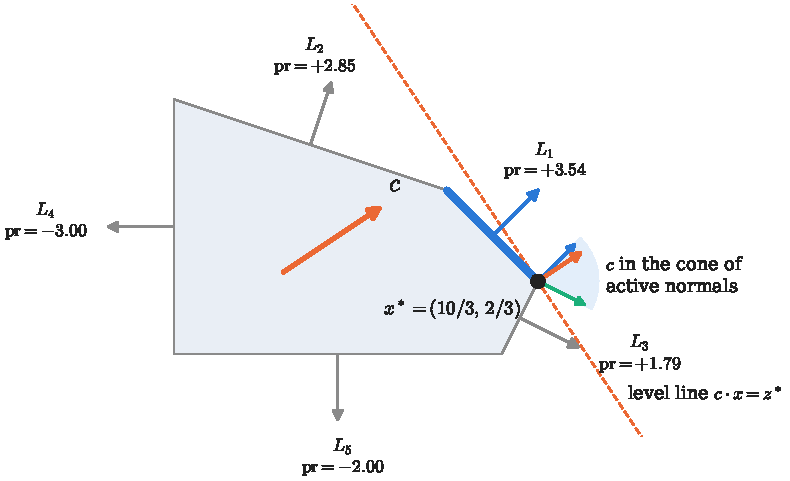
\includegraphics[width=0.78\linewidth]{figures/fig1_geometry.pdf}
  \caption{The geometric meaning of the method, for
  $\max\,3x+2y$ subject to $L_1\colon x+y\le4$, $L_2\colon x+3y\le7$, $L_3\colon 2x-y\le6$,
  $x,y\ge0$. Each face carries its outward normal and the projection $\mathrm{pr}$ of the
  objective vector $c$ onto that normal. The largest projection belongs to $L_1$ (blue), and
  $L_1$ indeed contains the optimum $x^*=(10/3,\,2/3)$. At $x^*$ the vector $c$ lies inside the
  cone spanned by the normals of the two active faces, $c=\tfrac73\,a_1+\tfrac13\,a_3$; these
  multipliers form the certificate of optimality.}
  \label{fig:geometry}
\end{figure}

The published method left two questions open. First, the selection rule is a heuristic, and
Grishin~\cite{grishin2008} notes that it may, ``with a certain probability'', pick a wrong face
and produce only a quasi-optimal point. When exactly is the method right? Second, the method
assumes that the object it looks for, a face containing the optimum, can always be found.
Can it?

\paragraph{Contributions.} This paper answers both questions and completes the method.
\begin{enumerate}[label=(\arabic*)]
  \item \textbf{Exact correctness criterion} (\cref{thm:run}). A run of the method returns an
  optimal point if and only if every hyperface it selects is principal in the problem it is
  selected from. A wrong choice can never be compensated later (\cref{thm:step}).
  \item \textbf{Principal hyperfaces exist} (\cref{cor:exists}). If the objective is non-zero,
  every optimal point lies on a principal hyperface with a usable pivot. This rests on Farkas'
  lemma, which we prove over an arbitrary ordered field by Fourier--Motzkin elimination
  (\cref{thm:farkas}), the same ``drop one dimension at a time'' idea that drives the method.
  \item \textbf{The selection rule is exact in the plane} (\cref{thm:plane}) and fails in three
  dimensions (\cref{prop:counter}), by an explicit, machine-checked counterexample.
  \item \textbf{A certified algorithm} (\cref{alg:certified}, \cref{thm:certified}). The
  method, augmented with a dual-certificate check and backtracking, always returns an optimal
  point when one exists. Every answer it certifies can be checked independently.
  \item \textbf{Machine-checked proofs.} Every result is formalised in Lean~4~\cite{lean4}
  with Mathlib~\cite{mathlib2020} (\cref{sec:lean}), and the worked example of
  \cite{grishin2008} is confirmed exactly (\cref{sec:examples}).
\end{enumerate}

We make no claim about worst-case speed. In the worst case the certified algorithm explores
exponentially many branches, as any exhaustive search may. Its value is a guarantee of
correctness together with a checkable proof for every answer.

% =====================================================================
\section{Setting and notation}\label{sec:setting}

Let $\K$ be a linearly ordered field, for example $\mathbb{Q}$ or $\R$. All results hold over
any such field, so in particular they hold in exact rational arithmetic. A \emph{linear program}
with $n$ variables and a finite index set $I$ of constraints is
\begin{equation}\label{eq:lp}
  \text{maximise } c\cdot x \quad\text{subject to}\quad a_i\cdot x\le b_i \quad (i\in I),
\end{equation}
with $c, a_i\in\K^n$ and $b_i\in\K$. A point $x$ is \emph{feasible} if it satisfies every
constraint, and \emph{optimal} if it is feasible and $c\cdot y\le c\cdot x$ for every feasible
$y$. Constraint $i$ is \emph{active} at $x$ if $a_i\cdot x=b_i$.

\begin{definition}[Principal hyperface]
Constraint $k$ is a \emph{principal hyperface} of \eqref{eq:lp} if it is active at some optimal
point.
\end{definition}

\begin{definition}[Redundancy]
Constraint $k$ is \emph{redundant} if every $x$ that satisfies all constraints $i\ne k$ also
satisfies constraint $k$.
\end{definition}

\begin{definition}[Projection rule]
Constraint $k$ has the \emph{largest projection} if $c\cdot a_k>0$ and
$(c\cdot a_k)/\|a_k\| > (c\cdot a_i)/\|a_i\|$ for every other $i$ with $c\cdot a_i>0$. To avoid
square roots, the formal statement compares
$(c\cdot a_i)^2\,\|a_k\|^2 < (c\cdot a_k)^2\,\|a_i\|^2$, which is equivalent for positive
projections.
\end{definition}

\begin{definition}[Elimination step]
Let $a_{kj}\ne0$. Replacing constraint $k$ by the equality $a_k\cdot x=b_k$ and solving it for
$x_j$ gives
\[
  x_j \;=\; \frac{1}{a_{kj}}\Bigl(b_k-\sum_{l\ne j} a_{kl}x_l\Bigr).
\]
Substituting into the objective and every constraint yields the \emph{reduced problem} in
$n-1$ variables, with
\[
  c'_l = c_l - \frac{c_j a_{kl}}{a_{kj}},\qquad
  a'_{il} = a_{il} - \frac{a_{ij}a_{kl}}{a_{kj}},\qquad
  b'_i = b_i - \frac{a_{ij}b_k}{a_{kj}} \qquad (l\ne j).
\]
The map $\mathrm{lift}$ inserts the forced value of $x_j$ back into a point of the reduced
problem (back substitution).
\end{definition}

\begin{figure}[t]
  \centering
  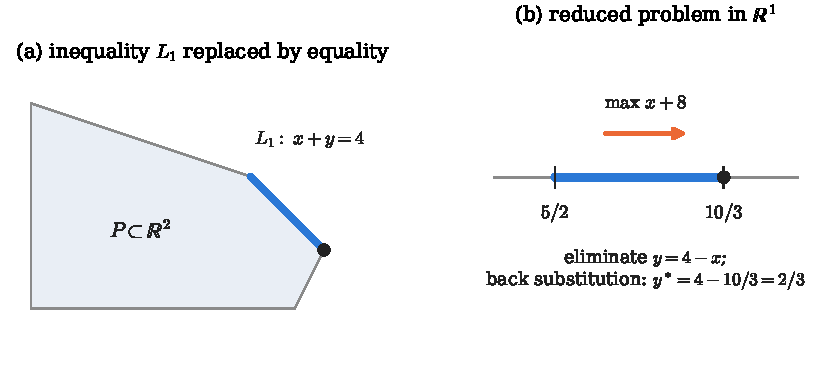
\includegraphics[width=0.92\linewidth]{figures/fig2_reduction.pdf}
  \caption{One step of the method on the example of \cref{fig:geometry}. (a)~The principal
  hyperface $L_1$ is turned into the equality $x+y=4$. (b)~Eliminating $y=4-x$ leaves the
  one-dimensional problem $\max\,x+8$ on $[5/2,\,10/3]$. Its optimum $x=10/3$ is lifted back by
  $y=4-x=2/3$.}
  \label{fig:reduction}
\end{figure}

% =====================================================================
\section{When is the method correct?}\label{sec:correctness}

\begin{theorem}[One step]\label{thm:step}
Let $a_{kj}\ne0$.
\begin{enumerate}[label=(\alph*)]
  \item A point $y$ is feasible for the reduced problem if and only if $\mathrm{lift}(y)$ is
  feasible for \eqref{eq:lp}. Every lifted point lies on the hyperface $a_k\cdot x=b_k$, and
  every point of that hyperface is a lifted point.
  \item If $k$ is principal and $y$ is optimal for the reduced problem, then $\mathrm{lift}(y)$
  is optimal for \eqref{eq:lp}. If $k$ is principal, the reduced problem has an optimal point.
  \item If $k$ is not principal, then $\mathrm{lift}(y)$ is not optimal, whatever $y$ is.
\end{enumerate}
\end{theorem}

\begin{proof}[Proof sketch]
The substitution identity $u\cdot\mathrm{lift}(y)=u'\cdot y+u_j b_k/a_{kj}$ holds for every
linear form $u$, which gives (a). The objective changes by a constant, so optimality transfers
between the problem restricted to the hyperface and the reduced problem. If $k$ is principal,
an optimum of \eqref{eq:lp} lies on the hyperface, which gives (b). Every lifted point is on the
hyperface, so an optimal lifted point would make $k$ principal, which gives (c).
\end{proof}

A \emph{run} of the method is a sequence of $n$ elimination steps with non-zero pivots,
followed by a feasible point of the resulting zero-dimensional problem, lifted back step by
step.

\begin{theorem}[Correctness criterion]\label{thm:run}
A run of the method returns an optimal point if and only if every hyperface it selects is
principal in the problem it is selected from.
\end{theorem}

\begin{proof}[Proof sketch]
By induction on $n$ using \cref{thm:step}(b) for ``if''. For ``only if'', an optimal lifted
point makes the chosen hyperface principal (\cref{thm:step}(c)), and the reduced point is then
optimal for the reduced problem.
\end{proof}

\Cref{thm:run} is the exact statement of when the Potapov--Grishin method is right: the
geometry of elimination is always sound, and only the choice of faces matters.

% =====================================================================
\section{Principal hyperfaces always exist}\label{sec:existence}

The method searches for principal hyperfaces. We now show that the search target exists. The
key tool is Farkas' lemma. The version of Mathlib used here provides it only in a topological
form for real inner-product spaces, so we prove the finite, algebraic form over an arbitrary
ordered field.

\begin{theorem}[Farkas' lemma over an ordered field]\label{thm:farkas}
A finite system $a_i\cdot x\le b_i$ over $\K$ either has a solution, or there are multipliers
$y_i\ge0$ with $\sum_i y_i a_i=0$ and $\sum_i y_i b_i<0$. Not both.
\end{theorem}

\begin{proof}[Proof sketch]
By induction on the number of variables, following Fourier and
Motzkin~\cite{motzkin1936,schrijver1986}. Eliminate the last variable by keeping the
inequalities in which it does not occur and adding every pair in which it occurs with opposite
signs, with positive weights that cancel it. A solution of the smaller system extends to a
solution of the original one: the pairwise sums guarantee that every lower bound for the
eliminated variable lies below every upper bound. A certificate for the smaller system pulls
back to one for the original system, because its rows are non-negative combinations of the
original rows.
\end{proof}

\begin{theorem}[Optimality conditions; strong duality at an optimum]\label{thm:kkt}
If $x$ is optimal, there are $y_i\ge0$, non-zero only on constraints active at $x$, with
$\sum_i y_i a_i=c$. Consequently a feasible point $x$ is optimal if and only if there is
$y\ge0$ with $\sum_i y_ia_i=c$ and $c\cdot x=\sum_i y_ib_i$.
\end{theorem}

The vector $y$ of \cref{thm:kkt} is a \emph{certificate of optimality}. It is easy to check, and
by weak duality it proves optimality regardless of how it was found. In \cref{fig:geometry} it
is $y=(\tfrac73,0,\tfrac13,0,0)$.

\begin{corollary}[Existence of principal hyperfaces]\label{cor:exists}
If \eqref{eq:lp} has an optimal point and $c\ne0$, then there are a principal hyperface $k$ and
an index $j$ with $a_{kj}\ne0$. So the method can always take a correct, non-degenerate step.
\end{corollary}

\begin{proof}
By \cref{thm:kkt}, $c=\sum_i y_ia_i$ with $y$ supported on active constraints. If every active
$a_i$ were zero, $c$ would be zero.
\end{proof}

% =====================================================================
\section{How good is the selection rule?}\label{sec:rule}

At an optimal vertex, $c$ lies in the cone spanned by the active normals (\cref{thm:kkt}). The
selection rule bets that the normal closest in angle to $c$ is one of them. The following
lemma makes the method's assumption ``no superfluous constraints''~\cite{grishin2008} precise
and says what non-redundancy rules out.

\begin{lemma}[Cone obstruction]\label{lem:cone}
If $a_k$ is a non-negative combination of normals of \emph{other} constraints that are all active
at a common feasible point, then constraint $k$ is redundant.
\end{lemma}

\begin{theorem}[The rule is exact in the plane]\label{thm:plane}
Let $n=2$ and suppose no constraint is redundant. If constraint $k$ has the largest projection,
then $k$ is active at every optimal point. In particular, $k$ is principal.
\end{theorem}

\begin{proof}[Proof sketch]
Write $p(v)=c\cdot v$ and $q(v)=c\times v$, the planar cross product. By \cref{thm:kkt},
$\sum y_i q(a_i)=0$ and $\sum y_ip(a_i)=\|c\|^2>0$ over the active normals. In these coordinates
the rule says $|q(a_k)|/p(a_k)<|q(a_i)|/p(a_i)$ for every active $a_i$ with $p(a_i)>0$, so $a_k$
makes a strictly smaller angle with $c$. If $q(a_k)\ge0$, some active $a_{i_2}$ lies strictly
on the same side of $c$ and beyond $a_k$, so $a_k$ is a non-negative combination of $c$ and
$a_{i_2}$, hence of active normals. If $k$ were inactive, \cref{lem:cone} would make it
redundant. The case $q(a_k)<0$ is symmetric. See \cref{fig:rule}(a).
\end{proof}

\begin{proposition}[The rule can fail in three dimensions]\label{prop:counter}
Consider $\max\,z$ subject to
\[
  L_1\colon x+z\le0,\quad L_2\colon -x+y+z\le0,\quad L_3\colon -x-y+z\le0,\quad
  L_4\colon 7y+10z\le1,\quad L_5\colon -z\le10.
\]
The feasible set is a bounded polytope with no redundant constraint, and its unique optimum is
the origin, where $L_1,L_2,L_3$ are active. The constraint $L_4$ has the largest projection,
$10/\sqrt{149}\approx0.819$ against $1/\sqrt2\approx0.707$ for $L_1$, but it is not principal.
So any run that starts with $L_4$ returns a non-optimal point.
\end{proposition}

\begin{figure}[t]
  \centering
  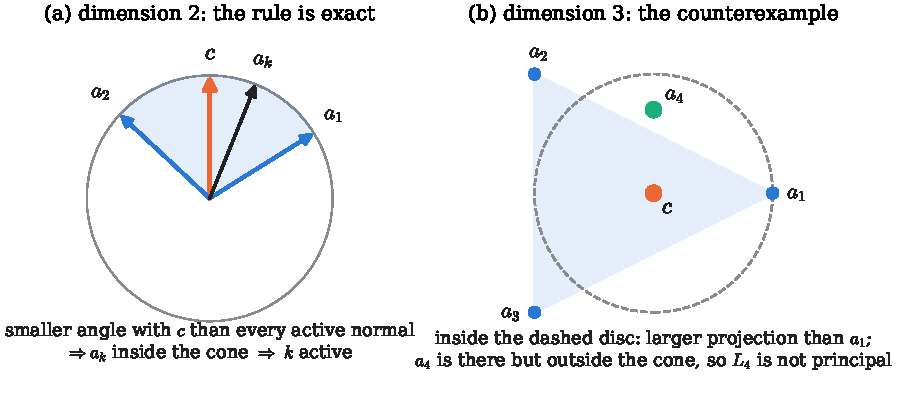
\includegraphics[width=0.94\linewidth]{figures/fig3_selection_rule.pdf}
  \caption{Why the projection rule is exact in the plane and not beyond. (a)~In dimension two,
  a normal $a_k$ that makes a smaller angle with $c$ than every active normal lies inside their
  cone; by \cref{lem:cone} it must be active. (b)~In dimension three (\cref{prop:counter}),
  normals are shown by their intersection with the plane at height one above $c=(0,0,1)$. The
  active normals $a_1,a_2,a_3$ span the shaded triangle. The dashed disc contains the normals
  with a larger projection than $a_1$. The normal $a_4$ is inside the disc but outside the
  triangle, so $L_4$ wins the rule without being principal.}
  \label{fig:rule}
\end{figure}

\begin{figure}[t]
  \centering
  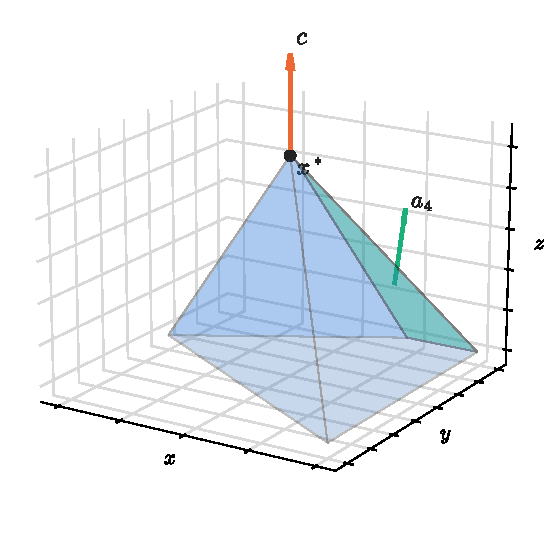
\includegraphics[width=0.62\linewidth]{figures/fig4_counterexample.pdf}
  \caption{The polytope of \cref{prop:counter}. The optimum is the apex at the origin, on
  $L_1,L_2,L_3$ (blue). The face $L_4$ (green) has the normal closest in direction to $c$, but
  it does not contain the optimum.}
  \label{fig:counter}
\end{figure}

% =====================================================================
\section{The certified principal hyperface method}\label{sec:certified}

\Cref{thm:run,cor:exists} suggest how to complete the method. Keep the projection rule as the
\emph{order} in which faces are tried. After each step, assemble a certificate of optimality
from the certificate of the reduced problem, check it, and stop as soon as it holds. When the
check fails, the chosen face was wrong (or the certificate is not unique), so backtrack to the
next face. The certificate for the current problem is assembled from the certificate $z'$ of
the reduced one by keeping $z'_i$ for $i\ne k$ and setting
\[
  z_k \;=\; \frac{1}{a_{kj}}\Bigl(c_j-\sum_{i\ne k} z'_i a_{ij}\Bigr).
\]

\begin{algorithm}[t]
\caption{Certified principal hyperface method, $\textsc{Solve}(P)$}\label{alg:certified}
\begin{algorithmic}[1]
\If{$P$ has no variables}
  \State \Return $(\varnothing,0)$ if $P$ is feasible, else \textsc{none}
\EndIf
\State order the constraints by decreasing projection $(c\cdot a_k)/\|a_k\|$
\For{each constraint $k$ in this order} \Comment{the selection rule}
  \State $j\gets$ index of the largest $|a_{kj}|$; \textbf{skip} $k$ if $a_{kj}=0$
  \State $(y,z')\gets\textsc{Solve}(\text{reduced problem of }P\text{ by }k,j)$
  \State $x\gets\mathrm{lift}(y)$;\quad $z\gets$ certificate assembled from $z'$
  \If{$x$ feasible, $z\ge0$, $\sum_i z_ia_i=c$, $c\cdot x=z\cdot b$}\label{line:check}
    \State \Return $(x,z)$ \Comment{certified optimal}
  \EndIf
\EndFor
\State \Return the feasible candidate with the largest objective \Comment{repair}
\end{algorithmic}
\end{algorithm}

\begin{theorem}[Certified method]\label{thm:certified}
For every linear program over an ordered field, \cref{alg:certified} terminates, and:
\begin{enumerate}[label=(\alph*)]
  \item every point it returns is feasible;
  \item if the problem has an optimal point, it returns an optimal point;
  \item whenever the check in line~\ref{line:check} succeeds, the returned certificate proves
  optimality.
\end{enumerate}
\end{theorem}

\begin{proof}[Proof sketch]
Termination is structural: recursion is on the number of variables, and each level considers
finitely many constraints. Part (a) follows from \cref{thm:step}(a). For (b), suppose an optimum
exists. If no certificate succeeds, the algorithm returns the best of all candidates. By
\cref{cor:exists} (or, when $c=0$, by moving to the boundary along a non-zero normal) some
principal face with a non-zero pivot is among them; by induction its branch returns an optimal
point of the reduced problem, which lifts to an optimal point (\cref{thm:step}(b)). Part (c) is
weak duality.
\end{proof}

\begin{remark}[Complexity]
In the worst case the backtracking explores exponentially many branches, so
\cref{alg:certified} is not a polynomial-time algorithm, and we do not claim otherwise.
Polynomial algorithms for linear programming are classical~\cite{khachiyan1979,karmarkar1984}.
The contribution here is different: the original geometric method, completed so that it is
always correct and every certified answer carries an independently checkable proof. On the
examples below, the first branch is accepted (\cref{sec:examples}).
\end{remark}

% =====================================================================
\section{Worked examples}\label{sec:examples}

\paragraph{The example of Grishin (2008).} The paper~\cite{grishin2008} solves
\[
\begin{aligned}
&\max\ 3x_1+4x_2+8x_3+5x_4+12x_5+2x_6 \quad\text{subject to}\\
&L_1\colon 3x_1+2x_2-x_3+6x_4+x_5+x_6\le24,\qquad L_2\colon x_1+6x_2+x_3+2x_6\le18,\\
&L_3\colon x_4+2x_5\le12,\qquad L_4\colon 3x_4+x_5\le12,\qquad L_5\colon 2x_1+x_2+x_3\le24,\\
&L_6\colon 2x_3+x_5+3x_6\le36,\qquad L_{6+j}\colon -x_j\le0\ \ (j=1,\dots,6),
\end{aligned}
\]
choosing the hyperfaces $L_3, L_2, L_6, L_{12}, L_8, L_4$, and reports
$x^*=(2.4,\,0,\,15.6,\,2.4,\,4.8,\,0)$ with $z^*=201.6$. We confirm in Lean that this point is
exactly optimal, with the certificate
\[
  y = \bigl(0,\ 3,\ \tfrac{47}{10},\ \tfrac1{10},\ 0,\ \tfrac52,\ 0,\ 14,\ 0,\ 0,\ 0,\ \tfrac{23}{2}\bigr),
  \qquad y\cdot b = \tfrac{1008}{5}=201.6,
\]
that every hyperface chosen in the paper is principal, and that the first choice $L_3$ has the
largest projection $29/\sqrt5$. \Cref{alg:certified} returns the same point and the same
certificate on its first branch.

\paragraph{The counterexample.} On the problem of \cref{prop:counter}, the projection rule
orders the constraints $L_4, L_1, L_2, L_3, L_5$. The single-pass method commits to $L_4$ and
fails. \Cref{alg:certified} also tries $L_4$ first, rejects it because the assembled certificate
is not valid, backtracks, and returns the origin with the certificate
$y=(\tfrac12,\tfrac14,\tfrac14,0,0)$.

% =====================================================================
\section{Formal verification in Lean 4}\label{sec:lean}

All definitions and theorems are formalised in Lean~4 (v4.35.0) with Mathlib, over an arbitrary
linearly ordered field. The development has about 1{,}600 lines in the library
\lean{PotapovSat.LP}. It contains no \lean{sorry}, no additional axioms and no
\lean{native\_decide}. For every main theorem, \lean{\#print axioms} reports only the three
standard axioms of Lean (\lean{propext}, \lean{Classical.choice}, \lean{Quot.sound}).
\Cref{tab:lean} maps the results of this paper to their formal names.

\begin{table}[ht]
\centering\small
\caption{Results of the paper and their names in the Lean development.}\label{tab:lean}
\begin{tabular}{@{}lll@{}}
\toprule
Result & Lean name & File \\
\midrule
\Cref{thm:step}(a) & \lean{Problem.feasible\_reduce\_iff} & \lean{LP/Elimination} \\
\Cref{thm:step}(b) & \lean{Problem.isOptimal\_lift} & \lean{LP/Elimination} \\
\Cref{thm:step}(c) & \lean{Problem.not\_isOptimal\_lift} & \lean{LP/Elimination} \\
\Cref{thm:run} & \lean{Run.isOptimal\_iff} & \lean{LP/Elimination} \\
\Cref{thm:farkas} & \lean{farkas}, \lean{solvable\_iff} & \lean{LP/Farkas} \\
\Cref{thm:kkt} & \lean{Problem.exists\_dual\_of\_isOptimal} & \lean{LP/Optimality} \\
 & \lean{Problem.isOptimal\_iff\_exists\_certificate} & \lean{LP/Optimality} \\
\Cref{cor:exists} & \lean{Problem.exists\_isPrincipal} & \lean{LP/Optimality} \\
\Cref{lem:cone} & \lean{Problem.redundant\_of\_mem\_activeCone} & \lean{LP/Redundancy} \\
\Cref{thm:plane} & \lean{Problem.active\_of\_isMaxProjection} & \lean{LP/Plane} \\
\Cref{prop:counter} & \lean{ProjectionCounterexample.*} & \lean{LP/Examples} \\
\Cref{thm:certified} & \lean{Problem.solve\_feasible}, \lean{Problem.solve\_isOptimal} & \lean{LP/Solver} \\
Example of~\cite{grishin2008} & \lean{Grishin2008.*} & \lean{LP/Examples} \\
\bottomrule
\end{tabular}
\end{table}

\Cref{alg:certified} is an executable Lean function. Its outputs on both examples of
\cref{sec:examples} are part of the build: if they ever changed, the build would fail. To
reproduce, install Lean with \texttt{elan} and run
\begin{lstlisting}
cd lean && lake exe cache get && lake build
\end{lstlisting}

% =====================================================================
\section{Python implementation}\label{sec:python}

The package \texttt{principal-hyperfaces} implements \cref{alg:certified} in exact rational
arithmetic and makes the same choices as the Lean function. Its test suite checks the two
examples of \cref{sec:examples} against the values verified in Lean, and checks 60 random bounded
problems against exhaustive vertex enumeration.

\begin{lstlisting}[language=Python]
from principal_hyperfaces import LinearProgram, solve

lp = LinearProgram.create(
    c=[3, 2],
    A=[[1, 1], [1, 3], [2, -1], [-1, 0], [0, -1]],
    b=[4, 7, 6, 0, 0])
sol = solve(lp)
print(sol.x, sol.value, sol.certified)   # (10/3, 2/3)  34/3  True
print(sol.dual)                          # (7/3, 0, 1/3, 0, 0)
\end{lstlisting}

% =====================================================================
\section{Conclusion}\label{sec:conclusion}

The principal hyperface method of Potapov and Grishin rests on a simple picture: the objective
vector points at the face that holds the optimum. We have shown exactly when this picture leads
to the right answer, that the face it looks for always exists, that the projection rule is
infallible in the plane but not in space, and how a certificate check with backtracking turns
the method into an algorithm that is always correct. All of it is machine-checked. Natural next
steps are a polynomial bound for well-conditioned classes of problems, and applications of the
certified method to discrete scheduling problems, where the same geometry of ``most constrained
first'' applies.

\section*{Data and code availability}
The Lean development, the Python package, and the scripts that generate the figures are
available at \repourl, under the MIT licence. This paper is distributed under the Creative
Commons Attribution 4.0 International licence (CC BY 4.0).

\section*{Acknowledgments}
The author used software tools, including an AI assistant, for technical help with the Lean
formalisation, the code and the English text. The research direction, the questions studied and
all decisions are the author's own. Every mathematical result is machine-checked in Lean~4.

% =====================================================================
\begin{thebibliography}{99}\small

\bibitem{potapov2007dep}
G.\,G.~Potapov and I.\,Yu.~Grishin.
Vyrishennya zadachi liniynoho prohramuvannya metodom poslidovnoho vyznachennya holovnykh
hipergraney [Solving the linear programming problem by sequential determination of principal
hyperfaces].
Deposited at the State Scientific and Technical Library of Ukraine; abstracted in
\emph{Deponovani naukovi roboty}, 2007, No.~1--2, 10~pp. (in Ukrainian).

\bibitem{grishin2007visnyk}
I.~Grishin and G.~Potapov.
Linear programming: a new polynomial-time algorithm.
\emph{Visnyk of the Volodymyr Dahl East Ukrainian National University}, 2007, No.~1(107),
pp.~113--119.

\bibitem{grishin2007riga}
I.~Grishin and G.~Potapov.
A new polynomial-time algorithm for linear programming.
In: \emph{The 5th International Conference ``Information Technologies and Management''
(IT\&M)}, Programme and Theses, Riga, 2007, pp.~45--46.

\bibitem{grishin2008}
I.\,Yu.~Grishin.
Evristicheskiy algoritm opredeleniya glavnykh graney pri reshenii zadachi lineynogo
programmirovaniya [Heuristic algorithm for determining principal faces in solving the linear
programming problem].
\emph{Vestnik NTU ``KhPI''. Informatika i modelirovanie}, 2008, No.~49, pp.~33--41 (in Russian).
\url{https://repository.kpi.kharkov.ua/handle/KhPI-Press/34736}

\bibitem{timirgaleeva2015}
R.\,R.~Timirgaleeva and I.\,Yu.~Grishin.
Novyy metod resheniya zadachi sovmestimosti lineynykh neravenstv v ekonomicheskikh zadachakh
planirovaniya raskhoda resursov [A new method for the compatibility problem of linear
inequalities in economic resource-planning problems].
\emph{Vestnik Mariyskogo gosudarstvennogo universiteta. Ser. Selskokhozyaystvennye nauki.
Ekonomicheskie nauki}, 2015, No.~1 (in Russian).

\bibitem{dantzig1963}
G.\,B.~Dantzig.
\emph{Linear Programming and Extensions}.
Princeton University Press, 1963.

\bibitem{kleeminty1972}
V.~Klee and G.\,J.~Minty.
How good is the simplex algorithm?
In: O.~Shisha (ed.), \emph{Inequalities III}, Academic Press, 1972, pp.~159--175.

\bibitem{khachiyan1979}
L.\,G.~Khachiyan.
A polynomial algorithm in linear programming.
\emph{Doklady Akademii Nauk SSSR} 244(5), 1979, pp.~1093--1096.

\bibitem{karmarkar1984}
N.~Karmarkar.
A new polynomial-time algorithm for linear programming.
\emph{Combinatorica} 4(4), 1984, pp.~373--395.

\bibitem{motzkin1936}
T.\,S.~Motzkin.
\emph{Beitr\"age zur Theorie der linearen Ungleichungen}.
Dissertation, University of Basel, 1936.

\bibitem{schrijver1986}
A.~Schrijver.
\emph{Theory of Linear and Integer Programming}.
Wiley, 1986.

\bibitem{lean4}
L.~de~Moura and S.~Ullrich.
The Lean 4 theorem prover and programming language.
In: \emph{Automated Deduction -- CADE 28}, LNCS 12699, Springer, 2021, pp.~625--635.

\bibitem{mathlib2020}
The mathlib Community.
The Lean mathematical library.
In: \emph{Proceedings of the 9th ACM SIGPLAN International Conference on Certified Programs and
Proofs (CPP 2020)}, 2020, pp.~367--381.

\end{thebibliography}

\end{document}
